\section{Approach}
We begin with a review of three foundation model families that utilize \textit{natural language supervision} differently: single-encoder classification pretraining, dual-encoder contrastive learning, and encoder-decoder image captioning. We then introduce Contrastive Captioners (CoCa) that share the merits of both contrastive learning and image-to-caption generation under a simple architecture. We further discuss how CoCa models can quickly transfer to downstream tasks with zero-shot transfer or minimal task adaptation.

\subsection{Natural Language Supervision}
\textbf{Single-Encoder Classification.}
The classic single-encoder approach pretrains a visual encoder through image classification on a large crowd-sourced image annotation dataset (\eg, ImageNet~\cite{deng2009imagenet}, Instagram~\cite{mahajan2018exploring} or JFT~\cite{zhai2021scaling}), where the vocabulary of annotation texts is usually fixed.
These image annotations are usually mapped into discrete class vectors to learn with a cross-entropy loss as
\begin{equation}
    \mathcal{L}_{\text{Cls}} = -p(y)\log q_{\theta}(x),
    \label{eq:main}
\end{equation}
where \(p(y)\) is a one-hot, multi-hot or smoothed label distribution from ground truth label \(y\).
The learned image encoder is then used as a generic visual representation extractor for downstream tasks.

\textbf{Dual-Encoder Contrastive Learning.}
Compared to pretraining with single-encoder classification, which requires human-annotated labels and data cleaning,
the dual-encoder approach exploits noisy web-scale text descriptions 
and introduces a learnable text tower to encode free-form texts.
The two encoders are jointly optimized
by contrasting the paired text against others in the sampled batch:
\begin{equation}
   \mathcal{L}_{\text{Con}} = -\frac{1}{N}
    (\underbrace{\sum_i^N\log{\frac{\exp(x_i^\top y_i / \sigma)}{\sum_{j=1}^{N} \exp(x_i^\top y_j / \sigma)}}}_\text{image-to-text} +
    \underbrace{\sum_i^N\log{\frac{\exp(y_i^\top x_i / \sigma)}{\sum_{j=1}^{N} \exp(y_i^\top x_j / \sigma)}}}_\text{text-to-image}),
\end{equation}
where \(x_i\) and \(y_j\) are normalized embeddings of the image in the $i$-th pair and that of the text in the \(j\)-th pair. \(N\) is the batch size, and \(\sigma\) is the temperature to scale the logits.
In addition to the image encoder,
the dual-encoder approach also learns an aligned text encoder that enables crossmodal alignment applications such as image-text retrieval and zero-shot image classification. Empirical evidence shows zero-shot classification is more robust~\cite{radford2021learning, jia2021scaling, andreassen2021evolution} on corrupted or out-of-distribution images.

\textbf{Encoder-Decoder Captioning.}
While the dual-encoder approach encodes the text as a whole,
the generative approach (\aka \ captioner) aims for detailed granularity and requires the model to predict the exact tokenized texts of \(y\) autoregressively.
Following a standard encoder-decoder architecture,
the image encoder provides latent encoded features (\eg, using a Vision Transformer~\cite{dosovitskiy2021an} or ConvNets~\cite{he2016deep}) and the text decoder learns to maximize the conditional likelihood of the paired text \(y\) under the forward autoregressive factorization:
\begin{equation}
    \mathcal{L}_{\text{Cap}} = - \sum_{t=1}^{T} \log P_{\theta}(y_{t}| y_{<t}, x).
\end{equation}
The encoder-decoder is trained with teacher-forcing~\cite{williams1989learning} to parallelize computation and maximize learning efficiency.
Unlike prior methods,
the captioner approach yields a joint image-text representation that can be used for vision-language understanding, and is also capable of image captioning applications with natural language generation.

\subsection{Contrastive Captioners Pretraining}
\label{secs:method}
\begin{figure}[t]
\centering
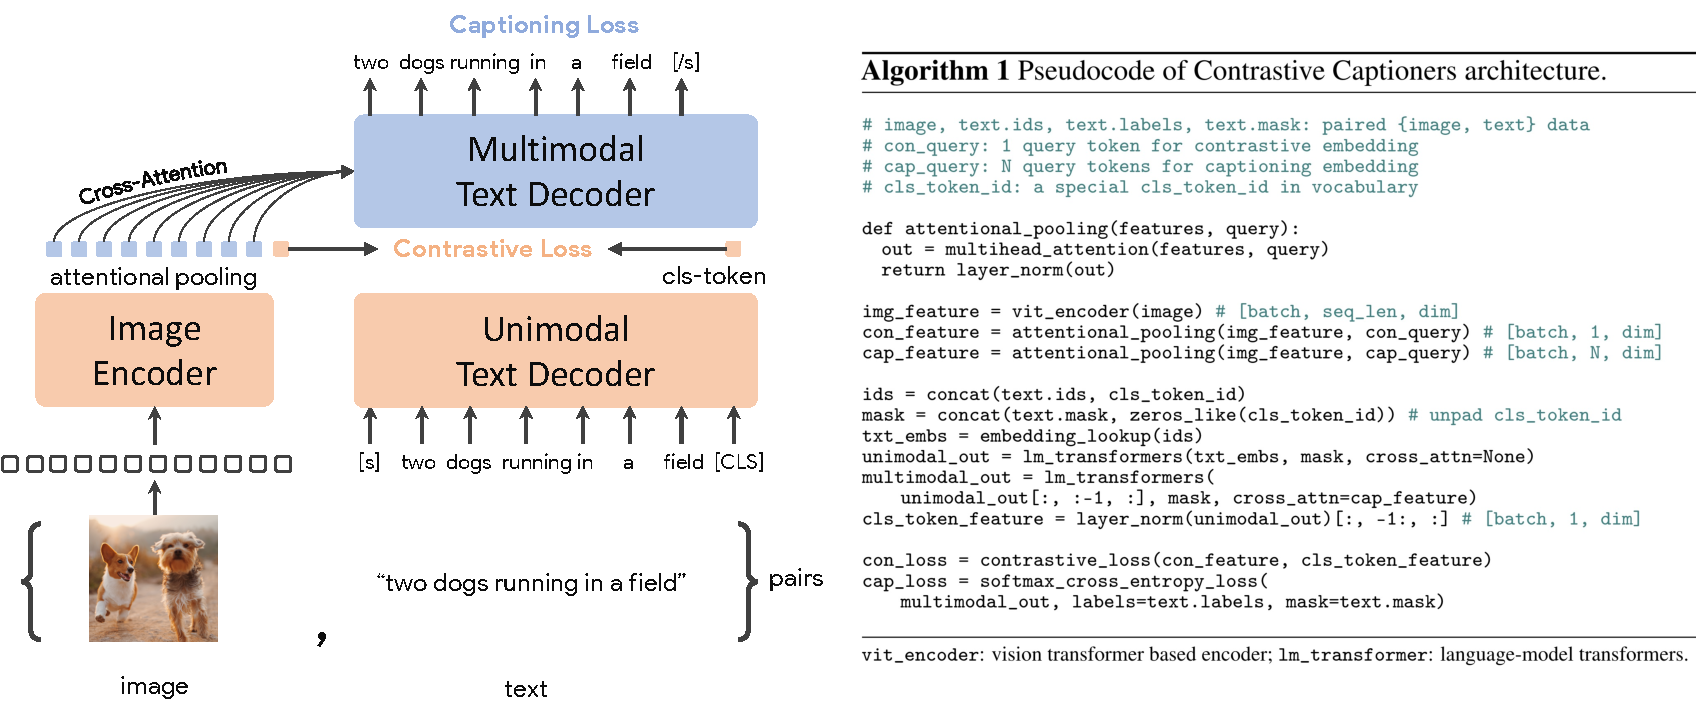
\includegraphics[width=\linewidth]{figures/coca_details}
\caption{Detailed illustration of CoCa architecture and training objectives.}
\label{figs:coca_details}
\end{figure}
Figure \ref{figs:coca_details} depicts
the proposed contrastive captioner (CoCa): a simple encoder-decoder approach that seamlessly combines the three training paradigms.
Similar to standard image-text encoder-decoder models,
CoCa encodes images to latent representations by a neural network encoder, for example, vision transformer (ViT)~\cite{dosovitskiy2021an} (used by default; it can also be other image encoders like ConvNets~\cite{he2016deep}), and decodes texts with a causal masking transformer decoder.
Unlike standard decoder transformers,
CoCa omits cross-attention in the first half of the decoder layers to encode \textit{unimodal} text representations,
and cascades the rest of the decoder layers, cross-attending to the image encoder for \textit{multimodal} image-text representations.
As a result, the CoCa decoder simultaneously produces both unimodal and multimodal text representations that allow us to apply both contrastive and generative objectives as
\begin{equation}
    \mathcal{L}_{\text{CoCa}} = \lambda_{\text{Con}} \cdot \mathcal{L}_{\text{Con}} + \lambda_{\text{Cap}} \cdot \mathcal{L}_{\text{Cap}},
    \label{eq:coca}
\end{equation}
where \(\lambda_{\text{Con}}\) and \(\lambda_{\text{Cap}}\) are loss weighting hyper-parameters.
We note that the single-encoder cross-entropy classification objective can be interpreted as a special case of the generative approach applied on image annotation data,
when the vocabulary is the set of all label names.

\textbf{Decoupled Text Decoder and CoCa Architecture.}
The captioning approach optimizes the conditional likelihood of text while the contrastive approach uses an unconditional text representation.
To address this dilemma and combine these two methods into a single model,
we propose a simple \textit{decoupled decoder} design where we split the decoder into unimodal and multimodal components,
by skipping the cross-attention mechanism in the unimodal decoder layers.
That is,
the bottom \(n_{\text{uni}}\) unimodal decoder layers encode the input text as latent vectors with causally-masked self-attention,
and the top \(n_{\text{multi}}\) multimodal layers further apply causally-masked self-attention and together with cross-attention to the output of the visual encoder.
All decoder layers prohibit tokens from attending to future tokens,
and it is straightforward to use the multimodal text decoder output for the captioning objective $\mathcal{L}_{\text{Cap}}$.
For the contrastive objective $\mathcal{L}_{\text{Con}}$,
we append a learnable \verb+[CLS]+ token at the end of the input sentence and use its corresponding output of unimodal decoder as the text embedding. We split the decoder in half such that $n_{\text{uni}}=n_{\text{multi}}$. Following ALIGN~\cite{jia2021scaling}, we pretrain with image resolution of 288$\times$288 and patch size 18\(\times\)18, resulting in a total of 256 image tokens.
Our largest CoCa model ("CoCa" in short) follows the ViT-giant setup in \cite{zhai2021scaling} with 1B-parameters in the image encoder and 2.1B-parameters altogether with the text decoder.
We also explore two smaller variants of ``CoCa-Base'' and ``CoCa-Large'' detailed in Table \ref{tabs:coca_variants}.


\begin{table}[t]
\centering
\small
\vspace{-2em}
\resizebox{1.0\textwidth}{!}{%
\begin{tabular}{@{}lcccccccccc@{}}
    \toprule
    & \multicolumn{3}{c}{Image Encoder} & \multicolumn{4}{c}{Text Decoder} & \multicolumn{2}{c}{Image / Text} & \\ 
    \cmidrule(lr){2-4} \cmidrule(lr){5-8} \cmidrule(lr){9-10}
    Model & Layers & MLP & Params & $n_{\text{uni}}$ & $n_{\text{multi}}$ & MLP & Params & Hidden & Heads & Total Params\\ 
    \midrule
    CoCa-Base & 12 & 3072 & 86M & 12 & 12 & 3072 & 297M & 768 & 12 & 383M \\
    CoCa-Large & 24 & 4096 & 303M & 12 & 12 & 4096 & 484M & 1024 & 16 & 787M \\
    \textbf{CoCa} & 40 & 6144 & 1B & 18 & 18 & 5632 & 1.1B & 1408 & 16 & 2.1B \\
 
    \bottomrule
  
\end{tabular}
}
\caption{\label{tabs:coca_variants} Size variants of CoCa. Both image encoder and text decoder are Transformers~\cite{dosovitskiy2021an, vaswani2017attention}.}
\end{table}

\textbf{Attentional Poolers.}
It is noteworthy that the contrastive loss uses a single embedding for each image while the decoder usually attends to a sequence of image output tokens in an encoder-decoder captioner \cite{wang2021simvlm}.
Our preliminary experiments show that a single pooled image embedding helps visual recognition tasks as a global representation,
while more visual tokens (thus more fine-grained) are beneficial for multimodal understanding tasks which require region-level features.
Hence,
CoCa adopts task-specific attentional pooling~\cite{lee2019set} to customize visual representations to be used for different types of training objectives and downstream tasks.
Here,
a \textit{pooler} is a single multi-head attention layer with $n_{\text{query}}$ learnable queries,
with the encoder output as both keys and values.
Through this,
the model can learn to pool embeddings with different lengths for the two training objectives, as shown in Figure \ref{figs:coca_details}.
The use of task-specific pooling not only addresses different needs for different tasks but also introduces the pooler as a natural task adapter.
We use attentional poolers in pretraining for generative loss \(n_{\text{query}}=256\) and contrastive loss \(n_{\text{query}}=1\).



\textbf{Pretraining Efficiency.}
A key benefit of the decoupled autoregressive decoder design is that it can compute two training losses considered efficiently.
Since unidirectional language models are trained with causal masking on complete sentences,
the decoder can efficiently generate outputs for both contrastive and generative losses with a single forward propagation (compared to two passes for a bidirectional approach \cite{li2021align}).
Therefore,
the majority of the compute is shared between the two losses and CoCa only induces minimal overhead compared to standard encoder-decoder models.
On the other hand, while many existing methods \cite{zhai2021lit,pham2021combined,singh2021flava,wang2021vlmo,li2021align,li2022blip} 
train model components with multiple stages on various data sources and/or modalities, CoCa is pretrained end-to-end from scratch directly with various data sources (\ie, annotated images and noisy alt-text images) by treating all labels as texts for both contrastive and generative objectives.


\subsection{Contrastive Captioners for Downstream Tasks}
\label{secs:downstream}

\textbf{Zero-shot Transfer.}
A pretrained CoCa model performs many tasks in a zero-shot manner by leveraging both image and text inputs, including zero-shot image classification, zero-shot image-text cross-retrieval, zero-shot video-text cross-retrieval. Following previous practices~\cite{radford2021learning, zhai2021lit}, ``zero-shot'' here is different from classical zero-shot learning in that during pretraining, the model may see relevant supervised information, but no supervised examples are used during the transfer protocol. For the pretraining data, we follow strict de-duplication procedures introduced in~\cite{jia2021scaling, zhai2021lit} to filter all near-domain examples to our downstream tasks.

\textbf{Frozen-feature Evaluation.}
As discussed in the previous section,
CoCa adopts task-specific attentional pooling~\cite{lee2019set} (\textit{pooler} for brevity) to customize visual representations for different types downstream tasks while sharing the backbone encoder.
This enables the model to obtain strong performance as a \textit{frozen encoder} where we only learn a new pooler to aggregate features. It can also benefit to multi-task problems that share the same frozen image encoder computation but different task-specific heads. As also discussed in ~\cite{he2021masked}, linear-evaluation struggles to accurately measure learned representations and we find the attentional poolers are more practical for real-world applications.

\begin{wrapfigure}{r}{0.42\linewidth}
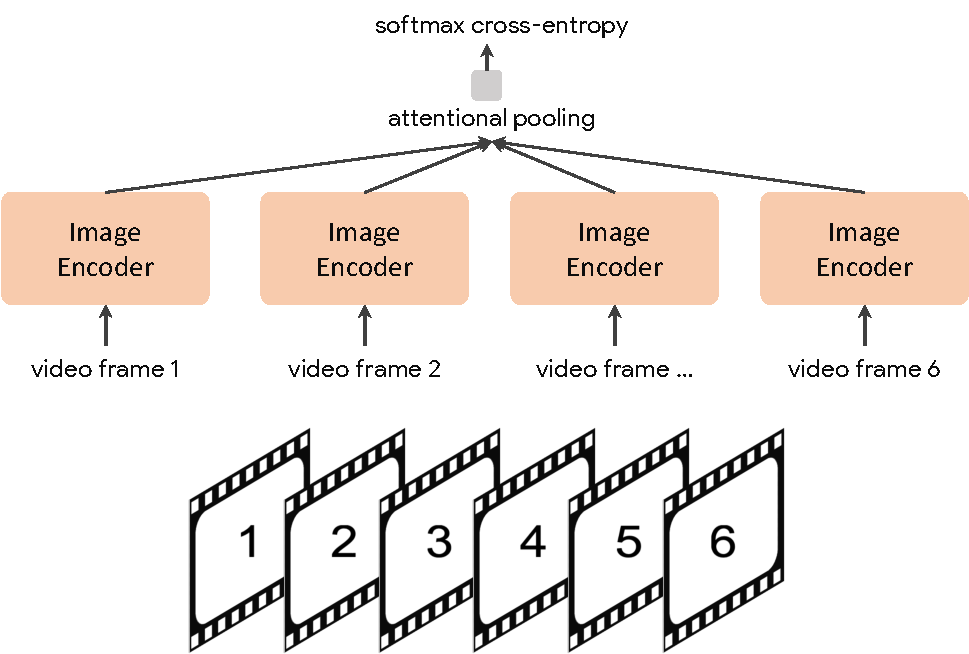
\includegraphics[width=\linewidth]{figures/coca_for_video}
\caption{CoCa for video recognition.}
\label{figs:coca_for_video}
\end{wrapfigure}
\textbf{CoCa for Video Action Recognition.} We use a simple approach to enable a learned CoCa model for video action recognition tasks. We first take multiple frames of a video and feed each frame into the \textit{shared} image encoder individually as shown in Figure~\ref{figs:coca_for_video}. For frozen-feature evaluation or finetuning, we learn an additional pooler on top of the spatial and temporal feature tokens with a softmax cross-entropy loss. Note the pooler has a single query token thus the computation of pooling over all spatial and temporal tokens is not expensive.
For zero-shot video-text retrieval, we use an even simpler approach by computing the mean embedding of 16 frames of the video (frames are uniformly sampled from a video).
We also encode the captions of each video as target embeddings when computing retrieval metrics.